%%%%%%%%%%%%%%%%%%%%%%%%%%%%%%%%%%%%%%%%%
% The Legrand Orange Book
% LaTeX Template
% Version 1.3 (21/8/13)
%
% This template has been downloaded from:
% http://www.LaTeXTemplates.com
%
% Original author:
% Mathias Legrand (legrand.mathias@gmail.com)
%
% License:
% CC BY-NC-SA 3.0 (http://creativecommons.org/licenses/by-nc-sa/3.0/)
%
% Compiling this template:
% This template uses biber for its bibliography and makeindex for its index.
% When you first open the template, compile it from the command line with the 
% commands below to make sure your LaTeX distribution is configured correctly:
%
% 1) pdflatex main
% 2) makeindex main.idx -s StyleInd.ist
% 3) biber main
% 4) pdflatex main x 2
%
% After this, when you wish to update the bibliography/index use the appropriate
% command above and make sure to compile with pdflatex several times 
% afterwards to propagate your changes to the document.
%
% This template also uses a number of packages which may need to be
% updated to the newest versions for the template to compile. It is strongly
% recommended you update your LaTeX distribution if you have any
% compilation errors.
%
% Important note:
% Chapter heading images should have a 2:1 width:height ratio,
% e.g. 920px width and 460px height.
%
%%%%%%%%%%%%%%%%%%%%%%%%%%%%%%%%%%%%%%%%%

%----------------------------------------------------------------------------------------
%	PACKAGES AND OTHER DOCUMENT CONFIGURATIONS
%----------------------------------------------------------------------------------------

\documentclass[11pt,fleqn, oneside]{book} % Default font size and left-justified equations

\usepackage[top=3cm,bottom=3cm,left=3.2cm,right=3.2cm,headsep=10pt,a4paper]{geometry} % Page margins

\usepackage{xcolor} % Required for specifying colors by name
\definecolor{ocre}{RGB}{240,0,0} % Define the orange color used for highlighting throughout the book

% Font Settings
\usepackage{avant} % Use the Avantgarde font for headings
%\usepackage{times} % Use the Times font for headings
\usepackage{mathptmx} % Use the Adobe Times Roman as the default text font together with math symbols from the Sym­bol, Chancery and Com­puter Modern fonts

\usepackage{microtype} % Slightly tweak font spacing for aesthetics
\usepackage[utf8]{inputenc} % Required for including letters with accents
\usepackage[T1]{fontenc} % Use 8-bit encoding that has 256 glyphs

% Bibliography
\usepackage[style=alphabetic,sorting=nyt,sortcites=true,autopunct=true,babel=hyphen,hyperref=true,abbreviate=false,backref=true,backend=biber]{biblatex}
\addbibresource{bibliography.bib} % BibTeX bibliography file
\defbibheading{bibempty}{}

\usepackage{tabularx}


% Index
\usepackage{calc} % For simpler calculation - used for spacing the index letter headings correctly
\usepackage{makeidx} % Required to make an index
\makeindex % Tells LaTeX to create the files required for indexing

%----------------------------------------------------------------------------------------

%----------------------------------------------------------------------------------------
%	VARIOUS REQUIRED PACKAGES
%----------------------------------------------------------------------------------------

\usepackage{titlesec} % Allows customization of titles

\usepackage{graphicx} % Required for including pictures
\graphicspath{{Pictures/}} % Specifies the directory where pictures are stored

\usepackage{lipsum} % Inserts dummy text

\usepackage{tikz} % Required for drawing custom shapes

\usepackage[english]{babel} % English language/hyphenation

\usepackage{enumitem} % Customize lists
\setlist{nolistsep} % Reduce spacing between bullet points and numbered lists

\usepackage{booktabs} % Required for nicer horizontal rules in tables

\usepackage{eso-pic} % Required for specifying an image background in the title page

%----------------------------------------------------------------------------------------
%	MAIN TABLE OF CONTENTS
%----------------------------------------------------------------------------------------

\usepackage{titletoc} % Required for manipulating the table of contents

\contentsmargin{0cm} % Removes the default margin
% Chapter text styling
\titlecontents{chapter}[1.25cm] % Indentation
{\addvspace{15pt}\large\sffamily\bfseries} % Spacing and font options for chapters
{\color{ocre!60}\contentslabel[\Large\thecontentslabel]{1.25cm}\color{ocre}} % Chapter number
{}  
{\color{ocre!60}\normalsize\sffamily\bfseries\;\titlerule*[.5pc]{.}\;\thecontentspage} % Page number
% Section text styling
\titlecontents{section}[1.25cm] % Indentation
{\addvspace{5pt}\sffamily\bfseries} % Spacing and font options for sections
{\contentslabel[\thecontentslabel]{1.25cm}} % Section number
{}
{\sffamily\hfill\color{black}\thecontentspage} % Page number
[]
% Subsection text styling
\titlecontents{subsection}[1.25cm] % Indentation
{\addvspace{1pt}\sffamily\small} % Spacing and font options for subsections
{\contentslabel[\thecontentslabel]{1.25cm}} % Subsection number
{}
{\sffamily\;\titlerule*[.5pc]{.}\;\thecontentspage} % Page number
[] 

%----------------------------------------------------------------------------------------
%	MINI TABLE OF CONTENTS IN CHAPTER HEADS
%----------------------------------------------------------------------------------------

% Section text styling
\titlecontents{lsection}[0em] % Indendating
{\footnotesize\sffamily} % Font settings
{}
{}
{}

% Subsection text styling
\titlecontents{lsubsection}[.5em] % Indentation
{\normalfont\footnotesize\sffamily} % Font settings
{}
{}
{}
 
%----------------------------------------------------------------------------------------
%	PAGE HEADERS
%----------------------------------------------------------------------------------------

\usepackage{fancyhdr} % Required for header and footer configuration

\pagestyle{fancy}
\renewcommand{\chaptermark}[1]{\markboth{\sffamily\normalsize\bfseries #1}{}} % Chapter text font settings
\renewcommand{\sectionmark}[1]{\markright{\sffamily\normalsize\thesection\hspace{5pt}#1}{}} % Section text font settings
\fancyhf{} \fancyhead[LE,RO]{\sffamily\normalsize\thepage} % Font setting for the page number in the header
\fancyhead[LO]{\rightmark} % Print the nearest section name on the left side of odd pages
\fancyhead[RE]{\leftmark} % Print the current chapter name on the right side of even pages
\renewcommand{\headrulewidth}{0.5pt} % Width of the rule under the header
\addtolength{\headheight}{2.5pt} % Increase the spacing around the header slightly
\renewcommand{\footrulewidth}{0pt} % Removes the rule in the footer
\fancypagestyle{plain}{\fancyhead{}\renewcommand{\headrulewidth}{0pt}} % Style for when a plain pagestyle is specified

% Removes the header from odd empty pages at the end of chapters
%\makeatletter
%\renewcommand{\cleardoublepage}{
%\clearpage\ifodd\c@page\else
%\hbox{}
%\vspace*{\fill}
%\thispagestyle{empty}
%\newpage
%\fi}

%----------------------------------------------------------------------------------------
%	THEOREM STYLES
%----------------------------------------------------------------------------------------

\usepackage{amsmath,amsfonts,amssymb,amsthm} % For including math equations, theorems, symbols, etc

\newcommand{\intoo}[2]{\mathopen{]}#1\,;#2\mathclose{[}}
\newcommand{\ud}{\mathop{\mathrm{{}d}}\mathopen{}}
\newcommand{\intff}[2]{\mathopen{[}#1\,;#2\mathclose{]}}
\newtheorem{notation}{Notation}[chapter]

%%%%%%%%%%%%%%%%%%%%%%%%%%%%%%%%%%%%%%%%%%%%%%%%%%%%%%%%%%%%%%%%%%%%%%%%%%%
%%%%%%%%%%%%%%%%%%%% dedicated to boxed/framed environements %%%%%%%%%%%%%%
%%%%%%%%%%%%%%%%%%%%%%%%%%%%%%%%%%%%%%%%%%%%%%%%%%%%%%%%%%%%%%%%%%%%%%%%%%%
\newtheoremstyle{ocrenumbox}% % Theorem style name
{0pt}% Space above
{0pt}% Space below
{\normalfont}% % Body font
{}% Indent amount
{\small\bf\sffamily\color{ocre}}% % Theorem head font
{\;}% Punctuation after theorem head
{0.25em}% Space after theorem head
{\small\sffamily\color{ocre}\thmname{#1}\nobreakspace\thmnumber{\@ifnotempty{#1}{}\@upn{#2}}% Theorem text (e.g. Theorem 2.1)
\thmnote{\nobreakspace\the\thm@notefont\sffamily\bfseries\color{black}---\nobreakspace#3.}} % Optional theorem note
\renewcommand{\qedsymbol}{$\blacksquare$}% Optional qed square

\newtheoremstyle{blacknumex}% Theorem style name
{5pt}% Space above
{5pt}% Space below
{\normalfont}% Body font
{} % Indent amount
{\small\bf\sffamily}% Theorem head font
{\;}% Punctuation after theorem head
{0.25em}% Space after theorem head
{\small\sffamily{\tiny\ensuremath{\blacksquare}}\nobreakspace\thmname{#1}\nobreakspace\thmnumber{\@ifnotempty{#1}{}\@upn{#2}}% Theorem text (e.g. Theorem 2.1)
\thmnote{\nobreakspace\the\thm@notefont\sffamily\bfseries---\nobreakspace#3.}}% Optional theorem note

\newtheoremstyle{blacknumbox} % Theorem style name
{0pt}% Space above
{0pt}% Space below
{\normalfont}% Body font
{}% Indent amount
{\small\bf\sffamily}% Theorem head font
{\;}% Punctuation after theorem head
{0.25em}% Space after theorem head
{\small\sffamily\thmname{#1}\nobreakspace\thmnumber{\@ifnotempty{#1}{}\@upn{#2}}% Theorem text (e.g. Theorem 2.1)
\thmnote{\nobreakspace\the\thm@notefont\sffamily\bfseries---\nobreakspace#3.}}% Optional theorem note

%%%%%%%%%%%%%%%%%%%%%%%%%%%%%%%%%%%%%%%%%%%%%%%%%%%%%%%%%%%%%%%%%%%%%%%%%%%
%%%%%%%%%%%%% dedicated to non-boxed/non-framed environements %%%%%%%%%%%%%
%%%%%%%%%%%%%%%%%%%%%%%%%%%%%%%%%%%%%%%%%%%%%%%%%%%%%%%%%%%%%%%%%%%%%%%%%%%
\newtheoremstyle{ocrenum}% % Theorem style name
{5pt}% Space above
{5pt}% Space below
{\normalfont}% % Body font
{}% Indent amount
{\small\bf\sffamily\color{ocre}}% % Theorem head font
{\;}% Punctuation after theorem head
{0.25em}% Space after theorem head
{\small\sffamily\color{ocre}\thmname{#1}\nobreakspace\thmnumber{\@ifnotempty{#1}{}\@upn{#2}}% Theorem text (e.g. Theorem 2.1)
\thmnote{\nobreakspace\the\thm@notefont\sffamily\bfseries\color{black}---\nobreakspace#3.}} % Optional theorem note
\renewcommand{\qedsymbol}{$\blacksquare$}% Optional qed square
\makeatother

% Defines the theorem text style for each type of theorem to one of the three styles above
\newcounter{dummy} 
\numberwithin{dummy}{section}
\theoremstyle{ocrenumbox}
\newtheorem{theoremeT}[dummy]{Theorem}
\newtheorem{problem}{Problem}[chapter]
\newtheorem{exerciseT}{Exercise}[chapter]
\theoremstyle{blacknumex}
\newtheorem{exampleT}{Example}[chapter]
\theoremstyle{blacknumbox}
\newtheorem{vocabulary}{Vocabulary}[chapter]
\newtheorem{definitionT}{Definition}[section]
\newtheorem{corollaryT}[dummy]{Corollary}
\theoremstyle{ocrenum}
\newtheorem{proposition}[dummy]{Proposition}

%----------------------------------------------------------------------------------------
%	DEFINITION OF COLORED BOXES
%----------------------------------------------------------------------------------------

\RequirePackage[framemethod=default]{mdframed} % Required for creating the theorem, definition, exercise and corollary boxes

% Theorem box
\newmdenv[skipabove=7pt,
skipbelow=7pt,
backgroundcolor=black!5,
linecolor=ocre,
innerleftmargin=5pt,
innerrightmargin=5pt,
innertopmargin=5pt,
leftmargin=0cm,
rightmargin=0cm,
innerbottommargin=5pt]{tBox}

% Exercise box	  
\newmdenv[skipabove=7pt,
skipbelow=7pt,
rightline=false,
leftline=true,
topline=false,
bottomline=false,
backgroundcolor=ocre!10,
linecolor=ocre,
innerleftmargin=5pt,
innerrightmargin=5pt,
innertopmargin=5pt,
innerbottommargin=5pt,
leftmargin=0cm,
rightmargin=0cm,
linewidth=4pt]{eBox}	

% Definition box
\newmdenv[skipabove=7pt,
skipbelow=7pt,
rightline=false,
leftline=true,
topline=false,
bottomline=false,
linecolor=ocre,
innerleftmargin=5pt,
innerrightmargin=5pt,
innertopmargin=0pt,
leftmargin=0cm,
rightmargin=0cm,
linewidth=4pt,
innerbottommargin=0pt]{dBox}	

% Corollary box
\newmdenv[skipabove=7pt,
skipbelow=7pt,
rightline=false,
leftline=true,
topline=false,
bottomline=false,
linecolor=gray,
backgroundcolor=black!5,
innerleftmargin=5pt,
innerrightmargin=5pt,
innertopmargin=5pt,
leftmargin=0cm,
rightmargin=0cm,
linewidth=4pt,
innerbottommargin=5pt]{cBox}				  
		  

% Creates an environment for each type of theorem and assigns it a theorem text style from the "Theorem Styles" section above and a colored box from above
\newenvironment{theorem}{\begin{tBox}\begin{theoremeT}}{\end{theoremeT}\end{tBox}}
\newenvironment{exercise}{\begin{eBox}\begin{exerciseT}}{\hfill{\color{ocre}\tiny\ensuremath{\blacksquare}}\end{exerciseT}\end{eBox}}				  
\newenvironment{definition}{\begin{dBox}\begin{definitionT}}{\end{definitionT}\end{dBox}}	
\newenvironment{example}{\begin{exampleT}}{\hfill{\tiny\ensuremath{\blacksquare}}\end{exampleT}}		
\newenvironment{corollary}{\begin{cBox}\begin{corollaryT}}{\end{corollaryT}\end{cBox}}	

%----------------------------------------------------------------------------------------
%	REMARK ENVIRONMENT
%----------------------------------------------------------------------------------------

\newenvironment{remark}{\par\vskip10pt\small % Vertical white space above the remark and smaller font size
\begin{list}{}{
\leftmargin=35pt % Indentation on the left
\rightmargin=25pt}\item\ignorespaces % Indentation on the right
\makebox[-2.5pt]{\begin{tikzpicture}[overlay]
\node[draw=ocre!60,line width=1pt,circle,fill=ocre!25,font=\sffamily\bfseries,inner sep=2pt,outer sep=0pt] at (-15pt,0pt){\textcolor{ocre}{R}};\end{tikzpicture}} % Orange R in a circle
\advance\baselineskip -1pt}{\end{list}\vskip5pt} % Tighter line spacing and white space after remark

%----------------------------------------------------------------------------------------
%	SECTION NUMBERING IN THE MARGIN
%----------------------------------------------------------------------------------------

\makeatletter
\renewcommand{\@seccntformat}[1]{\llap{\textcolor{ocre}{\csname the#1\endcsname}\hspace{1em}}}                    
\renewcommand{\section}{\@startsection{section}{1}{\z@}
{-4ex \@plus -1ex \@minus -.4ex}
{1ex \@plus.2ex }
{\normalfont\large\sffamily\bfseries}}
\renewcommand{\subsection}{\@startsection {subsection}{2}{\z@}
{-3ex \@plus -0.1ex \@minus -.4ex}
{0.5ex \@plus.2ex }
{\normalfont\sffamily\bfseries}}
\renewcommand{\subsubsection}{\@startsection {subsubsection}{3}{\z@}
{-2ex \@plus -0.1ex \@minus -.2ex}
{0.2ex \@plus.2ex }
{\normalfont\small\sffamily\bfseries}}                        
\renewcommand\paragraph{\@startsection{paragraph}{4}{\z@}
{-2ex \@plus-.2ex \@minus .2ex}
{0.1ex}
{\normalfont\small\sffamily\bfseries}}

%----------------------------------------------------------------------------------------
%	CHAPTER HEADINGS
%----------------------------------------------------------------------------------------

\newcommand{\thechapterimage}{}
\newcommand{\chapterimage}[1]{\renewcommand{\thechapterimage}{#1}}
\def\thechapter{\arabic{chapter}}
\def\@makechapterhead#1{
\thispagestyle{empty}
{\centering \normalfont\sffamily
\ifnum \c@secnumdepth >\m@ne
\if@mainmatter
\startcontents
\begin{tikzpicture}[remember picture,overlay]
\node at (current page.north west)
{\begin{tikzpicture}[remember picture,overlay]

\node[anchor=north west,inner sep=0pt] at (0,0) {\includegraphics[width=\paperwidth]{\thechapterimage}};

%Commenting the 3 lines below removes the small contents box in the chapter heading
\draw[fill=white,opacity=.6] (1cm,0) rectangle (8cm,-7cm);
\node[anchor=north west] at (1cm,.25cm) {\parbox[t][8cm][t]{6.5cm}{\huge\bfseries\flushleft \printcontents{l}{1}{\setcounter{tocdepth}{2}}}};

\draw[anchor=west] (5cm,-9cm) node [rounded corners=25pt,fill=white,fill opacity=.6,text opacity=1,draw=ocre,draw opacity=1,line width=2pt,inner sep=15pt]{\huge\sffamily\bfseries\textcolor{black}{\thechapter\ ---\ #1\vphantom{plPQq}\makebox[22cm]{}}};
\end{tikzpicture}};
\end{tikzpicture}}\par\vspace*{230\p@}
\fi
\fi
}
\def\@makeschapterhead#1{
\thispagestyle{empty}
{\centering \normalfont\sffamily
\ifnum \c@secnumdepth >\m@ne
\if@mainmatter
\startcontents
\begin{tikzpicture}[remember picture,overlay]
\node at (current page.north west)
{\begin{tikzpicture}[remember picture,overlay]
\node[anchor=north west] at (-4pt,4pt) {\includegraphics[width=\paperwidth]{\thechapterimage}};
\draw[anchor=west] (5cm,-9cm) node [rounded corners=25pt,fill=white,opacity=.7,inner sep=15.5pt]{\huge\sffamily\bfseries\textcolor{black}{\vphantom{plPQq}\makebox[22cm]{}}};
\draw[anchor=west] (5cm,-9cm) node [rounded corners=25pt,draw=ocre,line width=2pt,inner sep=15pt]{\huge\sffamily\bfseries\textcolor{black}{#1\vphantom{plPQq}\makebox[22cm]{}}};
\end{tikzpicture}};
\end{tikzpicture}}\par\vspace*{230\p@}
\fi
\fi
}
\makeatother % Insert the commands.tex file which contains the majority of the structure behind the template

\usepackage{wasysym}     
\newenvironment{checklist}{% JAMES ADDED!!
  \begin{list}{}{}% whatever you want the list to be
  \let\olditem\item
  \renewcommand\item{\olditem -- \marginpar{$\Box$} }
  \newcommand\checkeditem{\olditem -- \marginpar{$\CheckedBox$} }
}{%
  \end{list}
  }


\usepackage{pdfpages}

\begin{document}



%----------------------------------------------------------------------------------------
%	TITLE PAGE
%----------------------------------------------------------------------------------------


\includepdf[pages={1}]{wunderkarte.pdf}


%----------------------------------------------------------------------------------------
%	TABLE OF CONTENTS
%----------------------------------------------------------------------------------------

\chapterimage{chapter11.jpg} % Table of contents heading image

\pagestyle{empty} % No headers

\tableofcontents % Print the table of contents itself

\pagestyle{fancy} % Print headers again

%----------------------------------------------------------------------------------------
%	CHAPTER 1
%----------------------------------------------------------------------------------------

\chapterimage{yourmcr.jpg} % Chapter heading image

\chapter{Welcome to Jesus!}

Welcome to Jesus, and to one of the friendliest and most active Graduate communities in Cambridge. We hope that this Guide will give you all the information about the MCR, College, and Cambridge in general which you might need before you arrive. We have included a map of College and a map of Cambridge to help you orientate yourself. If there’s anything we’ve missed that you’d like to know, don’t hesitate to get in touch. In the meantime, good luck with the packing, and we look forward to meeting you!
\vspace{0.5cm}


\emph{From the Jesus College MCR Committee 2013-14}

\section{Your MCR Needs YOU!}

We hope to see you at as many MCR events as possible and please don’t hesitate to get in touch with us if you would like to get involved in organising an event. Elections are held at the end of May, but there are plenty of opportunities to help out before then. We will inform you of open positions on the Committee soon!
Sources of News and Information:

\begin{itemize}
\item ‘Living in Jesus’ Guide: it is important to read this in conjunction with our guide.  ‘Living at Jesus’ will be given to you upon arrival in Cambridge.
\item MCR Website: \url{http://mcr.jesus.cam.ac.uk}
\item MCR Facebook Group:  'Jesus College MCR’ – keep in touch and start discussions with other Graduates new and old!
	\url{https://www.facebook.com/groups/jesus.newgrads2011/}
\end{itemize}






 


\chapterimage{chapter2.jpg} % Chapter heading image

\chapter{The Jesus College MCR}

\section{Introduction}\index{Introduction}

The MCR (which stands for Middle Combination Room) is run solely by graduate students, for Graduates within Jesus College. Our aim is to represent the opinions and needs of the Graduate community to the College fellowship and the University, to maintain links with the Graduate Union and other MCRs, to facilitate the interaction of graduates with fellows, and perhaps most importantly to offer a wide range of social and academic opportunities targeted specifically towards the Graduate community. 

We offer an initial point of contact if you have problems with social or welfare issues and if we cannot help you directly we will refer you to the people who can. Throughout Freshers’ Fortnight, and the rest of the year, we hope to provide a varied selection of sports, academic and social events to suit all tastes. A number of exchange events will also be run in conjunction with the MCRs of other colleges, providing an opportunity to meet students outside Jesus College. The success of events organised by the society is only achieved thanks to an active and enthusiastic membership. If you have any ideas for other events or would like to help in the running of the MCR, please come and let us know.  

%------------------------------------------------

\section{MCR Committee 2013-14}\index{MCR Committee 2013-14}

See page~\pageref{comms}.

%---------------------------------------------Figure
\begin{figure}[!htbp]
\centering
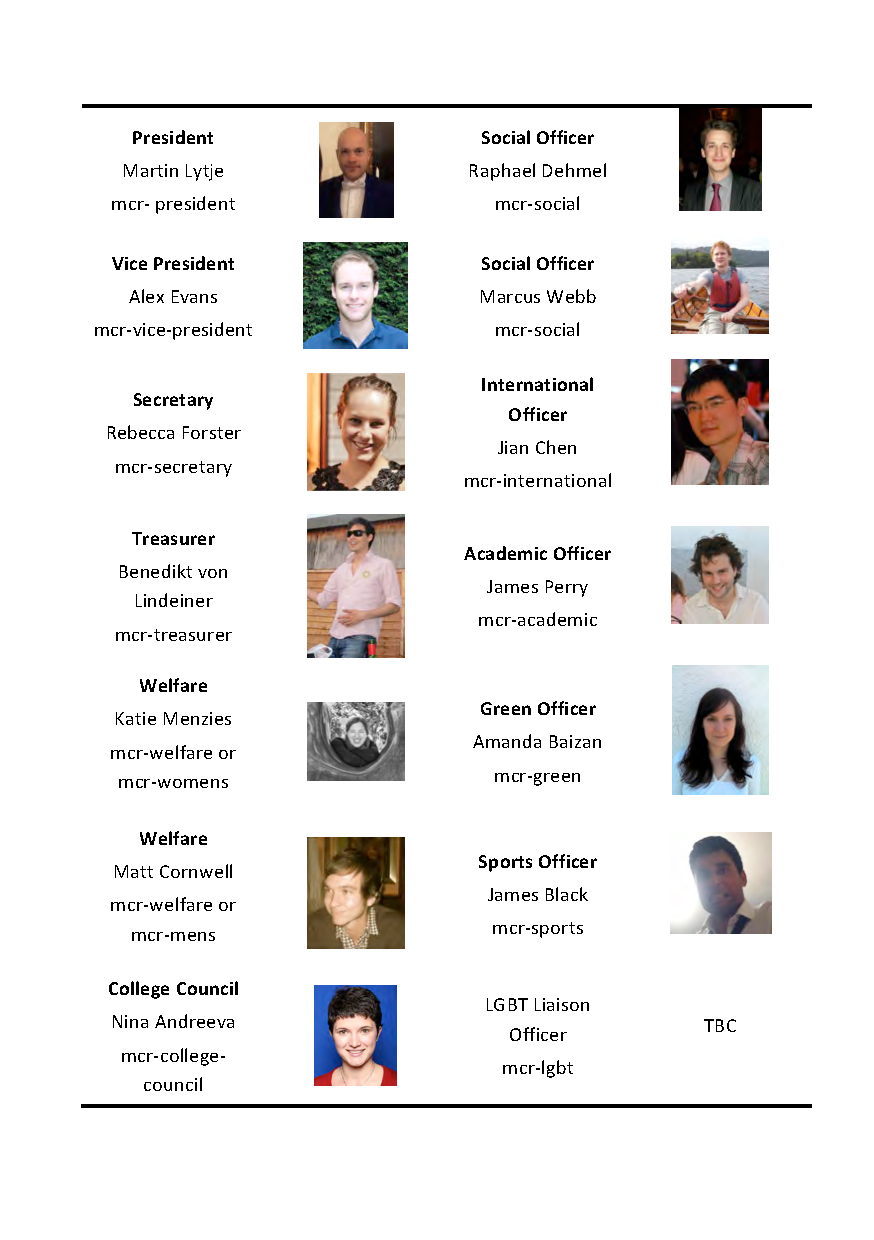
\includegraphics[width=\textwidth]{photoboard.pdf}
\caption{2013-14 committee members, add @jesus.cam.ac.uk to email prefixes below}
\label{comms}
\end{figure}


%------------------------------------------------

\section{Website, E-mail list, and Bulletins}\index{Website, E-mail list, and Bulletins}

The MCR keeps in touch with its members using an e-mail list; details of social events and other news are e-mailed to the list about once a week in the MCR Bulletin. We will endeavour to add all new Grads to the mailing list, but if for some reason you are not receiving the MCR bulletins, please register by contacting \url{mcr-vice-president@jesus.cam.ac.uk}.

The MCR has its own website: \url{http://mcr.jesus.cam.ac.uk}. On the site are full details of forthcoming events. If you have any questions, from punting to court booking or dining in college, that’s the place to look. The ‘Useful Links’ section (within the ‘Information’ section) provides a list of other useful websites about Cambridge. This Guide and these maps of Jesus College and Cambridge can be found on the site. There is also more useful information to be found so please do have a look at the website.

\section{Freshers' Fortnight }\index{Freshers' Fortnight}

Just before term starts in October, the MCR holds two weeks of social events. Everyone is welcome to attend; existing Grad students find them a welcome change from the work of the summer months, and for new Grads (Called ``Freshers'' in Cambridge), they are the perfect opportunity to meet people, have fun, and settle into Cambridge. The College system means that it’s really easy to meet people and make friends – it’s just up to you to make the most of all that’s on offer and to come to lots of the events we organise in Freshers’ Fortnight and throughout the year!    Remember that all new Grads will be in the same boat as you and that all current Grads remember what it was like to be a Fresher, so don’t be afraid to join in and meet the other Jesuans that make up the Graduate community.  

Many people will arrive on the weekend of the 28\textsuperscript{th} \& 29\textsuperscript{th} of September, and there will be events between Monday 30\textsuperscript{th} September and Sunday 13\textsuperscript{th} of October.  While MCR events start on the Monday (30\textsuperscript{th}), the college requires you to attend induction on the 4\textsuperscript{th} of October in order to matriculate into the college. This day concludes with a Special Grad Hall in the evening.  The committee members will be around so don’t hesitate to drop us an email, even if it is just to let us know that you are here!  If you plan to arrive early, please notify the Graduate Secretary, Sheena Bridgman (\url{s.bridgman@jesus.cam.ac.uk}), with as much advanced notice as possible to ensure that your room is ready upon arrival.

Regardless of when you arrive in Cambridge, feel free to join in with the Freshers’ Fortnight events when you get here – be assured that everyone arrives at different times throughout the two weeks and so every event is the perfect opportunity to meet people.  If you feel at all worried about turning up to an event alone, either e-mail one of the MCR committee beforehand and we can keep an eye out for you or come and introduce yourself to one of the committee members at the event, who should be  readily identifiable in colour co-ordinated matching t-shirts with our names on! 

During Freshers’ Fortnight, there are some events on offer that require Freshers’ to sign up/buy a ticket to in advance.

\subsection{Required to sign-up/buy ticket in advance}

Special Grad Hall on Friday 4\textsuperscript{th} October \& Grad Hall on Wednesday 2\textsuperscript{nd} of October and Wednesday 9\textsuperscript{th} October: You need to buy a ticket for these, using your University Card, from the machines in the Porters' Lodge or in East House, or by logging onto JNet and selecting ``Function Booking'' (more on JNet later).  If you have difficulty activating your card, please let us know in good time so we can try to help.   Also, please note that tickets can only be bought up to 3pm the day before the event.

An interesting event taking place just after Freshers’ Fortnight is Safari Night on Saturday 19\textsuperscript{th} October:  This is a great way to meet lots of people in an intimate setting. For \pounds{8} (bring your own wine) you get to eat your way from Grad house to Grad house through three courses, sampling the culinary expertise of your fellow students while sneaking a look at their houses. Sign up will be via an online payment. If you have trouble paying in this way please contact Ben, the treasurer, on \url{mcr-treasurer@jesus.cam.ac.uk}. If you would like to cook a meal for other grads then please contact Raphael and Marcus at \url{mcr-social@jesus.cam.ac.uk}.

Alongside the online booking, for some of the other events there will be sign-up sheets posted in the MCR Room – this gives us an idea of how many people will be coming, but it is sometimes fine to come along if you forget to sign up (the lists will remain on the notice board until 12 midday on the day of the event).  If you cannot sign up for these events using these sheets but still wish to come then please contact the Social Officers Raphael and Marcus on \url{mcr-social@jesus.cam.ac.uk}. Consult your Freshers’ Calendar for a list of these events.

Most MCR events are free, but for those for which you need to pay during Freshers’ Fortnight or throughout the year, you will usually be asked to use the online system or to leave a cheque in the pigeonhole of MCR Treasurer Ben von Lindeiner.  E-mail Ben (\url{mcr-treasurer@jesus.cam.ac.uk}) if you don’t have a chequebook and you can give him cash instead. 
There will also be opportunities during Freshers’ Fortnight to meet representatives from both Jesus and University Clubs/Societies. For more details about all Freshers’ events consult your Freshers’ Calendar or the MCR website.

If you will be arriving in Cambridge after Freshers’ Fortnight, don’t worry, you’ll still have plenty of opportunity to join in and meet everyone. There are lots of events throughout the year (see below). We will make sure you are welcomed and filled in on everything that has happened and all future events.  It doesn’t take long to find your feet and there are plenty of people willing to help you out. Again, just relax and join in; you’ll love it!

\section{MCR Events throughout the Year}

Every week there is a \textbf{Grad Hall}, held in Upper Hall (more on this later) – it’s a great way to break up the working week and socialise with friends or meet new people. We organise \textbf{International themed-nights} at some Grad Halls, which are always lots of fun – for example, last year we celebrated Thanksgiving, St Patrick’s Day and Australia Day among other general samplings of foreign cuisine. If you have an idea for a themed Grad Hall, get in touch with us! For those curious to mix with other Colleges, we also have \textbf{Exchange Halls} (called `swaps') to give you the chance to meet people from outside Jesus and see how things are done in other Colleges.  

In addition to weekly Grad Halls, we also hold \textbf{several larger dinner events} during the year, including our famous fancy-dress Halloween Party, our festive Christmas Party, the ever-popular Burns Night with Ceilidh and the magnificent End of Year Dinner.

The MCR also organises a number of additional events, such as \textbf{historical tours of College}, excursions to \textbf{neighbouring attractions}, and the \textbf{Graduate and Fellows Symposia}, which facilitate the informal intellectual integration between Grads and Fellows within Jesus College.  The focal point of academic life for Grads in College is the annual \textbf{Grads’ conference}, held this year on Saturday 15\textsuperscript{th} March 2014.  All Grads will be invited to present their research at the conference, which features a key-note speaker and conference dinner.

\section{The Grad Room}

The Grad Room is the central ‘hang-out zone’ for Graduate students. A great place to unwind with a newspaper and a cup of tea during the day, pre-dinner drinks on a Wednesday,  movie nights, and general socialising with other Grads. The Grad Room has a big TV (with Freeview), a DVD player, comfy sofas and a cool sound system! There is a nice kitchen with facilities for making tea and coffee, a fridge, a computer, and Eduroam Wi-Fi. We also have a selection of newspapers, magazines, fiction books from the library, board games, and croquet sets for your use.

Feel free to use the Grad Room for meeting friends, watching TV, reading the paper with a cup of coffee, etc – it’s essentially our living room and I’m sure you’ll come to think of it fondly after some happy times spent in there!
The Grad Room is on the left as you go through the archway between O and N staircases in Pump Court. Your University card will allow access via the security system. It is essential that the Grad Room is kept securely locked when not in use. Your card should be activated and working when you arrive; however, if you have any problems with access, see the Porters. 

\textbf{You can collect your mail from your personal pigeon hole in the Grad Room.}


It is best to use as your address:

\textbf{(Your name)}

\textbf{Jesus College}

\textbf{Cambridge}

\textbf{CB5 8BL}

This means that all your post will go to the Porters’ Lodge and the lovely Porters will then put the post in your pigeonhole.  It also means that any items that require a signature will be signed for in the P’Lodge meaning you don’t have to wait at home if you’re expecting a delivery.  The Porters will also forward your post to your new address if and when you leave Cambridge, which is unlikely to happen if you use an alternative address such as your College house.  College bills will also use Jesus College as your address, making it easier to provide proof of address .



%----------------------------------------------------------------------------------------
%	CHAPTER 2
%----------------------------------------------------------------------------------------

\chapterimage{chapter1.jpg} % Table of contents heading image

\chapter{Jesus College}

\section{Getting Started}

\subsection{What should I pack?}

Well, clothes are a good start. See “Social Life and College Sports” for more information about gowns, formal wear etc. Cambridge can get pretty cold in winter, so bring your woolly jumpers. A pillow and duvet (and probably a duvet cover) are provided, but you will need your own sheets, pillow covers and towels (and probably your own duvet cover, as the College ones tend to have seen better days). 

Grads coming from overseas will probably want to buy bedding and towels once you get here rather than lug it from home Argos on Fitzroy Street, Debenhams in the Grafton Centre and John Lewis on Regent Street as well as the large Tesco on Cheddars Lane (see City Centre map) all sell these items. As most of the shops close at 5.30PM, if you will be arriving later than this, you should bring something to get you through the first night.

Pots and pans, cutlery and crockery will be useful. You may find there is a fair amount of stuff in your kitchen that has been left by previous tenants. Otherwise, fairly cheap kitchenware is available at Sainsbury’s in the town centre, or at Asda or Tesco supermarkets a short walk outside town, and friendly housemates are usually willing to lend a saucepan or two!


\subsection{Arrival}

\textbf{You are strongly encouraged to be in residence in time for the induction day on Friday 4\textsuperscript{th} October}. 

If you are arriving from overseas, buses run 24 hours from all the main London airports to Cambridge (http://www.nationalexpress.com) at the Parkside bus stop, on the boundary of Parker’s Piece, approximately 10 minutes walk from College. If you are coming by train, a taxi from the station should cost around £6.50 although it can cost more if you arrive late at night.  There are also buses from the station to the city centre, on a somewhat erratic timetable.  Buses to the city centre leave from the bus stop on your right as you exit the station, and include the numbers 1 and 7.  If you are in any doubt, just ask the driver if he goes to the city centre.

\textbf{When you arrive, the first thing to do is go to the Porters’ Lodge} (P’lodge), the first door on your left as you go through the College’s main entrance (the tower at the end of the path known as the ‘Chimney’). Here you can leave your bags if you have them with you, and ask for directions to the \textbf{Graduate Secretary}, Sheena Bridgman’s Office, which is located in M Staircase, Second Court, Room 4 to sign your tenancy agreement and pick up your University Card.  You must then go back to the P’lodge to get the key for your room. You should also \textbf{check your pigeonhole} (in the MCR Room) and get any more information that may be there for you. You may be able to borrow a small trolley (the Porters can help you find one) to help move your things round to your room. Unload your stuff, say hello to your housemates, have a cup of tea and get ready to come to the next Freshers’ event.

Even if you will be arriving in the middle of the night, don’t despair; the \textbf{Porters are on duty 24 hours a day}. If you arrive after business hours, the Porters will be able to advise you on how to check into your room. If you arrive between midnight and 6am, the large wooden doors at the end of the Chimney will be closed, and you will need to use the night bell, which is a small button located on the left side of the archway.  Just press that and a Porter will come and let you in. If you have any difficulties, you can \textbf{telephone the Porters’ Lodge 24-hrs a day on 01223 339339}.

\subsection{Matriculation}

Important: the \textbf{University Statutes require those who are new to Cambridge to sign the Matriculation List}.  At 9.00am for those with surnames beginning A-K and 9.45am for those with surnames beginning L-Z the matriculation ceremony will take place in Upper Hall. The Graduate tutor, Tim Wilkinson, will welcome you with a short speech and then you will be asked to sign the matriculation register. You will also be asked to provide a passport (and visa where appropriate) for scanning. Those who cannot attend at that time are asked to call on Tim during opening hours during the first two weeks of Full Term. 

Following the matriculation ceremony a Freshers’ photograph will be taken in Chapel court – dress code for which is business attire (suit and tie) plus an appropriate university gown (see ‘Dress code — Academic and Social’ on page~\pageref{dress} for information on gown hire/purchase)

\subsection{University Card}

The University card is your student ID card throughout the university, and your library card for the University and many Departmental Libraries. \textbf{University cards should be available from the Graduate Secretary} (Sheena Bridgman, M Staircase, Second Court, Room 4) upon your arrival, and can be collected when you sign your tenancy agreement. If for any reason your card is not available when you arrive but you want to buy tickets for Hall contact the committee for help (the earlier you do this, the greater the likelihood that we can source you a ticket in time!).  It’s worth making a note of the number in the bottom left corner on the back of your card in case you lose it - you will usually be charged for a replacement card.

Your University card will open doors to almost all the fun places in College.  You just need to wave your wallet or bag in front of the sensor and the door will open, as if by magic.  It is used as an entry card to the Quincentenary Library, the Kwok Room (computer centre) and the Grad Room. The bar code on the back is used to take out library books.   
It is sometimes referred to as your “Caff card” because you can also use it to buy tickets for meals in College (Caff/Formals), including Grad Hall.  The current system works as a debit system where you have to put money on your card account before you can use it. When you buy food in caff, drinks in the bar, or a hall ticket at the ticket machine in the Porters’ Lodge or online through the booking system, the money will automatically be debited from your card account. So before you can do all of this you need to put money on your card - this can be done in a number of ways:
\begin{itemize}
\item By cash, cheque or debit card (but there is a minimum of £20 if you pay by card) at the Catering Accounts office in East House: opening times are: Monday to Friday: 8.30am-1.00pm and 2.15pm-5.00pm (closes at 4.00pm on Fridays)
\item By cash/cheque at the Bar (minimum £10 and in multiples of £10)
\item On JNet:  https://jnet.jesus.cam.ac.uk/   Select ‘services’ then ‘Simple Online Payment System (SOPS)’ and follow the instructions on the screen.
\end{itemize}




Married students can also get a special University Card for their spouse, which allows access around the University.  Speak to Louise Hind in the Senior Tutor’s office and she can help you arrange this.

%------------------------------------------------

\section{Important People and Places}
\subsection{Summary}

See the table on page~\pageref{important_people}.

\newcolumntype{L}[1]{>{\raggedright\arraybackslash}p{#1}} %my special column type! ragged right, rather than p which is justi

\begin{table}\footnotesize
\caption{\textbf{Summary of important contacts in college}}
\label{important_people}
    \begin{tabular}{L{2.5cm}L{2cm}L{2cm}L{6cm}}
    The Master                          & Professor Ian White             & The Master’s Lodge                      & The Master of College is a Very Important Person, so be on your best behaviour if you see him; however, he is very approachable so don’t be afraid to talk to him! If you get an invitation to meet with the master (e.g. for drinks as a second or third year PhD student), make every effort to attend and RSVP if you are unable to attend.  \\
    The President                       & Professor Helen Skaer           & Staircase P, Room 2A                    & Head of the Fellowship (the academic fellows of college)                                                                                                                                                                                                                                                                                        \\
    The Senior Tutor                    & Dr Geoff Parks                  & Staircase N, Room 1                     & He is responsible for the Junior members of College and besides his academic duties, he is in charge of parking permits.                                                                                                                                                                                                                        \\
    The Graduate Tutor (acting)         & Professor Tim Wilkinson         & Staircase F, Room 6                     & (see below)                                                                                                                                                                                                                                                                                                                                     \\
    Graduate Secretary                  & Sheena Bridgman                 & Staircase M, Room 4                     & Often your first point of contact with the Graduate Tutors. From whom you will receive your University card and your tenancy agreement.                                                                                                                                                                                                         \\
    The Dean of College                 & Dr Michael Edwards              & Staircase K, Room 4                     & Also known as the bad Dean: who is responsible for discipline and party permits. Surgery times on Monday 1.05-1.25pm and Wednesday 1.05-1.25pm.                                                                                                                                                                                                 \\
    The Chaplain and Dean of the Chapel & Rev'd John Hughes               & Staircase D, Room 1                     & You will probably meet John at MCR events – he is also a Tutorial Advisor and is available for advice on religious matters or otherwise.                                                                                                                                                                                                        \\
    The Senior Bursar                   & Sir Christopher Pratt           & East House                              & He oversees the College finances.                                                                                                                                                                                                                                                                                                               \\
    The Buildings Manager               & Ms Elizabeth Megson             & East House                              & She is in charge of maintenance work and making sure all the buildings are kept in good working order.                                                                                                                                                                                                                                          \\
    The Manciple                        & Mrs Lisa Brown                  & Staircase J                             & She is in charge of catering and booking College rooms, and also oversees Housekeeping.                                                                                                                                                                                                                                                         \\
    The Financial Tutor                 & Dr Duncan Kelly                 & Staircase N, Room 1                     & He is responsible for all matters relating to financial hardship: applications to Access Funds, Supplementary Maintenance Committee, the General Scholarship Fund and other special College funds, as well as making special arrangements for paying your College bills.                                                                        \\
    The Porters                         & Head Porter—Mr. Grahame Appleby & Porters’ Lodge                          & Source of useful information, in charge of security, as well as looking after your post.  Contact in case of emergency (01223) 339339                                                                                                                                                                                                           \\
    The College Nurse                   & Ms. Jacky Poskitt               & Staircase I Library Court               & She will assist/advise/administer medical treatment. She manages the twice weekly physiotherapy clinics, and can refer you to other medical professionals when necessary.                                                                                                                                                                       \\
    Head of Housekeeping                & Mrs Claire Andrews              & Housekeeping Office (Vehicle Exit Gate) & First point of contact regarding problems with furniture (bed, wardrobe, etc.) before the Senior Bursar. Also who you talk to if you have problems with your bedders (cleaners).                                                                                                                                                                \\
    ~                                   & ~                               & ~                                       & ~                                                                                                                                                                                                                                                                                                                                               \\
    \end{tabular}
\end{table}

\subsection{The Graduate Tutors}

\textbf{Professor Tim Wilkinson, as the acting Graduate Tutor}, has primary responsibility for Graduates, and is the person to approach with any problems that may arise during your time at Jesus. Tim is located in F staircase, Room 6 or you can reach him at tdw13@cam.ac.uk. Arrangements can be made to see Prof. Wilkinson outside of normal hours by approaching the Graduate Secretary, Sheena Bridgman, by email (\url{gradtutor@jesus.cam.ac.uk}) or by phone on (01223) 339421. Prof. Wilkinson usually attends the grads and fellows high tables on Tuesday nights, so this is a good time to meet him.

\textbf{Sheena Bridgman, who is the Graduate Secretary}, can be found during office hours (Monday to Friday: 10.30am-12.30pm and 2.30-4.00pm) in M Staircase, Second Court, Room 4. Her telephone number is (01223) 339421 and her e-mail is \url{gradtutor@jesus.cam.ac.uk}. Application forms for grants from research funds for travel and other expenses can be obtained from her, together with documentary confirmation of Graduate student status for such matters as immigration and travel. Sheena is also in charge of Graduate accommodation, and is a useful person to know. 

\subsection{Tutorial Advisers}

In addition, there are a number of Fellows who are “Tutorial Advisers”. Graduate students may turn to any of the Tutorial Advisers for advice on any matter whatsoever and on any problems, great or small. They will provide a confidential and sympathetic ear and can direct you towards appropriate professional or expert advice if necessary. The Tutorial Advisers hold regular Tutorial hours when you can call in to see them; however, there is always a Tutorial Adviser on call, twenty-four hours a day in Term time, to deal with problems that cannot wait until the next advertised Tutorial hour. They can be contacted in case of an emergency or urgent problem, whatever the hour, via the Porter’s Lodge (01223 339339).  A list of the current Tutorial Advisers is pigeonholed to all students at the start of each year, and is posted on the notice boards outside the P’lodge. 

During Vacation periods, Graduate students should contact the Graduate Tutor by email or call on either Sheena Bridgman or Dr Geoff Parks (the Senior Tutor) in the Tutorial Office (01223 339468) during normal office hours.  If you find yourself in need of help urgently out of office hours, then you can phone the Porters’ Lodge.

\subsection{College Contacts}
Upon your arrival in College, \textbf{you will be assigned a College Contact who is a Fellow of Jesus College}. Your contact will be from your faculty or a related subject area. The role of your contact is to provide an informal and friendly point of contact within the College Fellowship should you need some simple advice. This role exists as a backup to your main ports of call through either your supervisor or the College Tutorial Advisors, or you may wish to discuss academic or professional matters of the sort not normally covered by your faculty supervisor or the College Tutorial Advisors. The second role of your contact is to support the social engagement of new Graduate students in the College. This is done in a variety of ways, and may include an invitation from your contact to attend undergraduate events in College, or an invitation(s) to separate Graduate only events. 

The College Contact Program is now entering its fifth year. It was received well by both the Fellowship and the Graduate students in its first four years and we hope you will you will find it a useful scheme. If you have any problems contacting your College contact or other issues, please contact the welfare officers Katie and Matt (\url{mcr-welfare@jesus.cam.ac.uk}) or Prof. Tim Wilkinson (\url{tdw13@cam.ac.uk}).  

\subsection{The Porters and the Porters’ Lodge}

The Porters ‘live’ in the Porters’ Lodge (P’lodge) at the end of the “Chimney” (see map attached). As your first point of contact with the College, the Porters are a great source of knowledge and are definitely the people to ask when you don't know something. The telephone number of the P’Lodge is (01223) 339339 – useful to know in an emergency, for example if you or one of your housemates burns the toast and sets off the fire alarm, the Porters will come round and turn it off, saving you from the noise (if not the embarrassment!)

The Porters will even give you new light bulbs (free of charge). You can leave stamped mail with the Porters for posting (although there is a mail box at the end of the Chimney on Jesus Lane). Internal mail for other people at Jesus can be left in their pigeonholes or with the Porters. Mail for Fellows and Officers of other Colleges or departments of the University can also be left with the Porters for free distribution via the UMS (University Mail Service). Mail to students in other Colleges can also be sent free of charge, via the ICMS (Inter-Collegiate Mail Service), which is a bit slower than UMS. There are trays for these two services in the P’lodge, and mail should be marked “UMS” or “ICMS” accordingly. Your mail will go into your pigeonhole in the Grad Room, and is delivered twice daily Mondays through Saturdays at around 8.30am and 12.30pm, so please check your pigeon hole from time to time.

Amongst the key personalities that you will need to know in the P’lodge are Grahame Appleby, who is the Head Porter, and Adam Fawkes, who is in charge of registering bicycles.  Get to know the Porters; most are very likeable and you will need their help sooner or later. In a sense they are the “power behind the throne” in terms of practical influence in College. In addition, at the P’Lodge you can check out the keys to the music and snooker rooms, tennis and squash courts, borrow a squash racquet, and book your tickets to formal halls and other events. 

\subsection{East House/Bursary}

East House is where you need to go to pay College bills, or fees, or to pick up grant or scholarship cheques.  The finance office is on the first floor on the left, and is open Monday to Thursday: 2:30pm-4:30pm (around the time bills are due, these hours are exteded to 10:00am-12:30pm and 2:30pm-4:30pm Monday to Friday).

\subsection{College Council}

This is not really a person or a place, but it is worth a mention and fits this category more than the others!  It is the decision making board of College, where any important changes to most aspects of the College (from building work to provision for students) are agreed upon. It meets fortnightly and feeds off recommendations made by lots of different committees, many of which are attended by Graduate representatives from the MCR committee. Council approves everything that happens in and to College, and minutes are available in the library and on JNet, the College’s intranet. There are four Junior representatives on Council: The JCSU President, one elected undergraduate rep, the MCR President and one elected Graduate rep.  This year’s Graduate Rep is yet to be confirmed at the time of writing of this handbook but once you arrive he/she can be contacted on \url{mcr-college-council@jesus.cam.ac.uk}. If you have any questions about Council, or an issue you would like to see raised, please get in touch with the council rep. 

\section{Accommodation}

\subsection{Overview}

Jesus College has all kinds of accommodation for Graduates. The largest house accommodates 16 people and the smallest houses, three. The College also owns some flats for couples and families, and in couples’ flats you won’t have to share communal space.  All accommodation is close to the College, usually on Jesus Lane, Maid’s Causeway, Malcolm Street or on Park Street and Lower Park Street. Rooms are graded according to their size, with most rooms possessing a washbasin. You will need to bring your own sheets, duvet covers and pillowcases (see ‘What should I pack?’), but a duvet and pillow (and possibly a duvet cover) are provided. Facilities vary, but all housing comes with all the necessary appliances to cook for yourself (ovens, hotplates, etc).  Some houses have microwaves, kettles and toasters but these will belong to a community spirited member of that house or have been left behind by some previous householder. Check out \url{mcr.jesus.cam.ac.uk} to see photos of the grad accommodation.

Fridge space is never sufficient – however, don’t panic, most of us have become minimalists and manage to fit our stuff onto one shelf of a fridge, and it encourages us to have a hearty meal at least once a week by going to grad hall!
Space is not a feature of most kitchens and none of the houses have common rooms, however, all houses with the exception of Little Trinity (16 Jesus Lane) have a small kitchen table where you can entertain guests, you just have to make the obvious arrangements with your housemates. When the weather is fine outdoor entertaining is the way to go, as many houses have small gardens. You may have guests stay overnight in your room, and fold-up beds are available from the Porters Lodge for a small nightly fee.

Almost all of the College’s housing has been renovated recently, but if you have any issues with your allocated room, see Sheena Bridgman. If any furniture in your room needs replacing or you are missing essential items, contact Mrs Claire Andrews in the housekeeping office (\url{c.andrews@jesus.cam.ac.uk}). For repairs you can fill in an online maintenance slip on JNet (explained later).

Most Graduate accommodation has a cleaner (known as a ‘bedder’) who comes in at least once a week to clean the communal areas (toilets, bathrooms, kitchens), while you are left to clean your own room yourself. For your safety, houses are equipped with a fire alarm system. \textbf{If the fire alarm is set off for any reason (e.g. burnt toast!), don’t panic – evacuate the building and call the Porters on (01223) 339339} and one of them will come round and turn it off. 

There has been a recent change to the College smoking policy following from the national ban on smoking in public spaces such as pubs and restaurants. As such, you are not permitted to smoke within the College grounds, except within two designated smoking areas (North Court car park; and shelter beside the electrical substation by Library Court).

\subsection{Laundry Facilities}

Over the summer of 2003 the College installed washing machines (and dryers in the larger houses) in all College Houses on Jesus Lane, Park St, Lower Park St, Malcolm Street and Maid’s Causeway (known as “external staircases”).  All Graduate accommodation is in these houses, so you should now be able to use these for most things rather than having to use the laundries within college.  If you need to use a tumble dryer, laundry facilities are available in College in the basement of Chapel Court 14. The laundries get busy—late at night is a good way to avoid queuing. Be Warned: If you are not there when your cycle ends, another person in line may remove your washing and dump it somewhere in the laundry, not necessarily on a clean surface! If you require the occasional use of an iron, one can be signed out from the P’lodge. There are ironing boards in the College launderettes or often left behind by previous tenants in many of the houses. 

\subsection{Car Parking}

The College is usually quite happy for your visitors to park in the College car park, although it is worthwhile checking with the Porters beforehand in case the College is expected to be busy. \textbf{If you wish to keep your own car in Cambridge, there are an extremely limited number of permits available to park in the College car park}. These are decided by ballot: \textbf{applications are made via the Senior Tutor's Office} (a parking permit will set you back £146 per term). If you do not park in College you will need a resident's parking permit from the Guildhall and a Pass from the University—the Senior Tutor will advise you on this. There are roads which do not require a permit on the other side of the river, which is fine on a temporary basis, but your car will be picked up and towed away, and you will be heavily fined, if you park it in the wrong place or illegally, so be careful!

\chapterimage{chapter3.jpg} % Chapter heading image
\chapter{Social Life and College Sports}
\section{Food and Drink}
\subsection{Graduate Hall}

Grad Hall is held \textbf{each Wednesday evening} throughout the year at 7.30pm in Upper Hall, and often outside term time too. It is preceded by drinks at 7pm in the Grad Room. It is a really good social occasion, providing an excellent mid-week escape from thoughts of the library or the lab. Everyone is welcome at the drinks, regardless of whether you’re attending Hall. Grad Hall is a great place to meet new friends from Jesus; it is also a chance to invite friends out for a meal. If you wish to meet a fellow or your supervisor away from the pressure of work then Grad Hall is a good place to find out what they are really like. 

Dinner is of High Table standard (i.e. what the Fellows are fed that evening): three courses followed by cheese and biscuits, coffee and mints, and port. It’s one of the best value and most delicious halls in Cambridge!  Wine is not provided, so please bring your own drinks (wine, beer and cider are all ok). Grads and their guests are afterwards encouraged to retire to the College Bar. 

\textbf{Tickets for Grad Hall must be purchased before 3pm the day before} from the ticket machines in the P’lodge or East House using your University card, or by making a function booking on JNet. These events are popular so you should really try to buy tickets as early as possible so as not to be disappointed.

We also organise exchange halls (see below) and international themed-nights at some Grad Halls, which are always lots of fun and give our international students a chance to share their culture – for example, in the past we have celebrated Thanksgiving, Australia Day, Chinese New Year, St Patrick’s Day and an African evening. If you have an idea for a themed Grad Hall then get in touch with us!

\subsection{College Bar}

The College bar is a little bit cheaper than town pubs. It opens at 6.30pm and serves until around 11pm on Sunday, Monday and Tuesday nights, 11.30pm on Wednesday and Thursday nights and until midnight on Fridays and Saturdays.  It’s worth taking the time to talk to James and the rest of the staff, as they are (nearly) always very friendly and take a real interest in what we are up to. They have asked us to remind you that Jesus bar is a “Members Only” facility (on account of the licence), which means that your guests will only be served if you are with them. There are several games available within the bar including table football, a TV, a Nintendo Wii, and sometimes an XBox. The bar looks like a trendy London bar, but the difference is that after you’ve been here a while you’ll be able to go in there most nights and find someone you know to have a chat with. 

\subsection{Caff, Formal Hall and High Table}

The more adventurous Graduates (and the domestically inept) take the opportunity to eat in the College cafeteria. \textbf{Lunch and dinner are both available daily} and the hours of opening can be found on the notice board next to the Hall. The food varies in quality but it is reasonably priced. Vegetarian and vegan food is always available on request. Caff opening hours during term time are: 
\begin{itemize}
\item Lunch: 		12.15pm-1.45pm		Monday to Friday
\item Dinner:		5.45pm-6.45pm 		Monday to Sunday 
\item Brunch: 	11.30am-1.30pm 		Saturdays only
\item Carvery lunch: 	12pm-1.30pm 			Sundays only
\end{itemize}


\textbf{On all evenings, except Monday and Saturday, Formal Hall also occurs}. This is a formal dining occasion and so \textbf{all College members must wear gowns}, and smart dress on Sundays. You receive a three-course meal, although wine is not provided. Tickets for Formal Hall can be purchased using the ticket machine in the P’lodge and East House, or by making a function booking on JNet, and must be bought before 3pm on the day before the dinner. All meals are paid for using your University card.

\textbf{On Tuesday evenings in term-time, Grads are invited to dine with the Fellows at High Table} (which is on the raised platform at the far end of the Hall) rather than on the main floor with the undergraduates. It costs a little more, but the service and quality of the food is higher and wine and a cheese course are also included. Pre-dinner drinks are served in the Fellows’ quarters and there is free port from the Fellows’ cellars at the end of the meal.  Numbers are very restricted, so you will have to be quick off the mark.

As Graduates at Jesus, we are not required to pay a Kitchen Fixed Charge (KFC). You can opt to pay KFC, which will make Caff and formal hall marginally cheaper, but most Grads do not find this cost effective. 

\subsection{Swaps}
We organise Exchange Formal Halls to other Colleges, which are the perfect opportunity to meet people from outside Jesus, to explore the many different characters of the Colleges, and to try out the food while you’re there - good for the curious amongst us! If there’s somewhere you would really like to go, then let us know!   Formal hall swaps are usually advertised in the weekly MCR bulletin, with sign-ups as directed, either via the social secretaries or the MCR website.

\section{Dress code — Academic and Social}
\label{dress}

There are dress codes for a variety of academic and social occasions in Cambridge. \textbf{“Academic” or “formal”} dress requires that gowns be worn, however they are only required for a few academic and College occasions, e.g. the Matriculation photograph, Graduate and Fellows Dinner, and graduation. They are also required for Formal Hall, although not for Grad Hall, and so many Graduates do not buy one.

A brand new gown will cost £85-£125 depending on your previous degree from Ryder \& Amies (22, Kings Parade – see Cambridge Map).  Other places to buy gowns and College branded clothing are Ede \& Ravenscroft (71-72, Trumpington St) and A.E. Clothier (5A, Pembroke St). On Tuesday 1st October from 11.30am to 12.30pm, the MCR will be selling ex-hire gowns at a reduced price. 

Gowns can also be hired from the GU shop (open 10am-5pm, Monday–Friday: to make a reservation call 01223 333312 or email hire@gradunion.cam.ac.uk) at £6 per day, as some of you will likely not need one very often. If you are planning to hire a gown for the Induction Day, then book early as there are a limited number and there will be a high demand.  It is also worth noting that if you have a black gown from another University you will probably get away with wearing it.

\textbf{“Black Tie”} means a Dinner Jacket (aka Tuxedo) for men, and an evening dress/cocktail dress for women. Dark suits are fine, but you will get plenty of wear out of a DJ, and you should certainly bring it with you if you own one. “Formal” dress usually means something you would call smart. Appropriate national/ethnic costume may be worn at most social events. 

Please remember though that for all MCR events turning up is more important than wearing the right clothes! We would rather see you there, no matter what you choose to wear, than have you sitting at home feeling like Cinderella. 

\section{JCSU}

\textbf{As a Graduate at Jesus, you are also a member of the JCSU} (Jesus College Student Union).  JCSU events are aimed at all students within College, both undergraduates and Graduates, and the MCR and JCSU work together on issues affecting all students. The JCSU also organises social activities which are aimed primarily at the undergraduates, but don’t be afraid to join in their cheesy discos (bops). Keep an eye on their notice boards at the bottom of caff steps to find out what’s going on, as well as information about other College societies including music, drama, and sport.  You can also see their website: \url{http://www-jcsu.jesus.cam.ac.uk/}. 

\section{Clubs and Societies}

Grads participate in all aspects of College life, and societies welcome (and often depend upon) Grad members, even though many of the organisers are undergrads. \textbf{The College Sports and Societies fair will be on Sunday 6th October}, this will give you an opportunity to find out more about what’s on offer and sign up for any that strikes your fancy.  Many of these will hold a ‘squash’ early in the term, which is an event to tell potential new members what they do – you can find out when these will be at the sign-up. See the JCSU website for a full list of clubs and societies, and there are notices and information on the P’lodge notice blackboards and at the bottom of the steps leading to the dining hall. 

\section{College Sports}

Jesus has an excellent sporting tradition and houses a great variety of sporting facilities on its own College ground, including football and cricket pitches, rugby field, squash hall, gym, tennis courts and not far from the College, our boathouse. Grads are an important part of many of the College Sports teams: from football to rowing to Ultimate Frisbee, there’s something for all abilities, whether you’d like to carry on with a sport you’ve been doing for years, or fancy trying something new. 

In addition to the many JCSU clubs and societies, the Grads also run our own socially orientated football and cricket teams, and the Jesus College Boat Club is always on the lookout for potential Grad talent. Having said that, it is up to you to decide what teams we form and so you should get in touch the committee if you would to join an existing team or suggest a new one.

On a more informal basis, Grads can often be found playing pick-up games of a variety of sports on a Sunday afternoon as part of the informal Sunday Sports Society. Be it football, American football, Aussie rules, rounders, or wiffleball, Sunday sporting is a good excuse for a bit of a laugh while getting some fresh air away from the books or the lab. Experience is definitely not a prerequisite—half of the fun is watching your fellow team mate handle a ball/bat/play a game he/she has never played before. 
You can participate in virtually any type of sport in the University too - the University teams will have stands at the Societies' Fair held on the 8th and 9th of October. For more information visit \url{http://www.cusu.cam.ac.uk/societies/fair/}. 
 
\chapterimage{chapter4.jpg} % Chapter heading image

\chapter{Computing and Library}

\section{College Computing}

\subsection{Facilities}

The College has some of the best computing facilities of any Cambridge College and a fantastic IT department. The Quincentenary library houses the Kwok Computer Room, which contains about 25 PCs running Windows7, as well as laser printers, a colour printer and a scanner. There is a small charge (added to your next bill) levied for printing: 4p (A4) and 8p (A3) per sheet for the laser printer and 12p for the colour printer.  Because the Kwok room is located within the Library proper, you must undergo a library induction (see below) to activate your access (University) card.

To get started, you will need to go to the IT department to get your username and password (which is your login for both the computers in the Kwok room and JNet).  The IT department is located in Library Court, Staircase I, and the opening hours are 9.00am-1.00pm and 2.30pm-5.30pm, Monday to Friday.  

The IT Department has a team of IT specialists, including a dedicated User Support Officer, Rob Spragg, who is on hand to answer questions and resolve any problems.  They will even have a look at your computer and try to fix it if it goes wrong.  In term-time, official user-support hours are from 14.30 to 17.30, Monday to Friday. During this period any computer-related queries are accepted.  You can contact the IT Department via e-mail \url{it-support@jesus.cam.ac.uk}, or by telephone at (01223) 339945. If you need assistance outside normal hours, you should e-mail your query to \url{it-support@jesus.cam.ac.uk}, which directs your query to all those working in the IT Department. 

\subsection{Network Connection}

All rooms in and round College have a socket on the College computer network. Connect your PC or Mac to the socket to give you access to the College network and the Internet direct from your room.  The cost of this is incorporated into your accommodation price.  You can get a network cable from the IT department if you do not already have one. 

For a new network connection to be established the IT department will need to know the physical address of your network adapter (often referred to as a MAC address). Every network adapter has a unique number associated with it similar in idea to the chassis number found on all cars. This MAC address is used by our new NAT firewall to identify a legitimate connection. For the firewall to be able to allow your machine access to the network it must know about your network adapter, hence the need for it to be registered with the IT Department.

Follow the instructions below to find the MAC address of your computer, then register it by visiting the following webpage
\url{https://jnet.jesus.cam.ac.uk/services/macreg.html} 

You can access this from your computer before you have registered, but you will need your JNet password to do so. Alternatively, go to the IT department in Library Court I.

Wireless is also in the process of being installed in college accommodation with many houses already setup with this service. Contact the IT department for more information if required.

How to find the MAC address of your computer’s network adapter:
\begin{itemize}
\item \textbf{Mac OSX:}
\begin{enumerate}
 \item Open SYSTEM PREFERENCES 
\item Select NETWORK
\item Select ETHERNET
\item Open the ADVANCED TAB 
\item The MAC address is the “Ethernet ID”
\end{enumerate}
\item \textbf{Windows XP / VISTA / 7:}
\begin{enumerate}
 \item Open CONTROL PANEL
\item Select NETWORK or NETWORK AND SHARING CENTRE 
\item  Select ETHERNET 
\item Select DETAILS
\item The MAC address is the “Physical Address”
\end{enumerate}
 
\end{itemize}

Your machine may automatically configure itself for the new network configuration, but if it doesn’t, then you can visit the IT department for support.
 
\subsection{JNet}
JNet is the College intranet and has loads of useful information on it – meal times and menus, information about College computing, the opening hours of College offices, and Staff names and contact details.  Your username and password are the same as for the Kwok Room – just drop into the IT department and they will tell you what yours are.  JNet is being used more and more, so it’s worth logging on and having a look around!  
 
Maintenance requests are handled on JNet – click on the square blue icon on the navigation bar and this will open a fault report.  You can order more furniture, report a leaky roof, report problems with your heating etc.  
 
It is also possible to pay your College Bill and put money on your University card (\pounds{20} minimum) on JNet – go to Money->Online Payments
   
\section{Hermes and your University email address}
   
Hermes is the system used for your University email address, which you will be automatically provided with.  Your email address will look like xxxxx@cam.ac.uk, where xxxxx is your CRS identifier issued by the Computing Service, and consists of your initials followed by a number.  You can find out your CRS-ID before you arrive – go to \url{http://www.cam.ac.uk/cs/new-students/newpgmail.html}. 
You can get your login name and initial password for Hermes and PWF through the Jackdaw system, by going to \url{https://jackdaw.cam.ac.uk/signup/}, and following the instructions through.  You will have to enter your admissions reference code issued by the Board of Graduate Studies and you should be able to do this within a couple of weeks of being offered a place.
Hermes mail can be accessed using any Web browser; this facility (Hermes Webmail) is particularly convenient if you are temporarily away from Cambridge.  You can login at \url{https://webmail.hermes.cam.ac.uk/}.  For further information see \url{http://www.cam.ac.uk/cs/docs/email.html}. 
   
\section{Public Workstation Facility (PWF)}
   
The Public Workstation Facility (PWF) is for the use of all staff and students of Cambridge University, and provides networked PCs and Apple Macintosh computers running a wide range of software, together with printers and scanners and a central file-store. The PCs in certain PWF rooms can run under the Linux operating system as an alternative to the standard Windows XP. 
Access to the PWF is from a number of public rooms and also from many Colleges and some Departments. Some of these institutions run their own computer rooms with special arrangements for access to the PWF; an increasing number have rooms managed in conjunction with the Computing Service (the PWF Managed Cluster Service).
   
All students are given PWF accounts when they join the University. You can get your login name and initial password for PWF and Hermes through the Jackdaw system, by going to \url{https://jackdaw.cam.ac.uk/signup/}, and following the instructions through.  You will have to enter your admissions reference code issued by the Board of Graduate Studies and you should be able to do this within a couple of weeks of being offered a place. 
   
\section{Zeus}
   
The JCSU has provided a server for the benefit of all students in College. This machine, called Zeus, runs Linux, and provides a wealth of useful services including website hosting and email lists. Zeus’s new webpage contains a growing collection of information \url{http://zeus.jesus.cam.ac.uk/} and user notes are currently located at: \url{http://www-jcsu.jesus.cam.ac.uk/computing/}. There is also a specific page about creating a website: \url{http://www-jcsu.jesus.cam.ac.uk/computing/writing-html.php}
To get an account on Zeus, just email the list of Zeus administrators at \url{zeus-admin@jesus.cam.ac.uk} (contact \url{mcr-vice-president@jesus.cam.ac.uk} for more information). You will then be able to log in and create your personal website. If you run a society, you can have a society website and society e-mail lists set up. 
   
\section{Raven}
   
Raven is the University of Cambridge's central web authentication service. Web-based services throughout the University may use Raven when they need to know who is using them.  For example, to sign up to events such as exchange halls on the MCR website, you have to sign in to ensure that only members of Jesus College have access.
   
If you have an account (and know your password) on the Hermes mail system, the Engineering Department mail system, or on the Biological Sciences 'Mole', collect your Raven password by visiting: \url{https://jackdaw.cam.ac.uk/get-raven-password}. 
   
If you are collecting a Raven password for the first time, or are re-collecting the original password allocated to you, not having changed it meanwhile, then you will be given the password immediately on the screen. If you have changed your Raven password since it was originally issued, then a new password will be generated and sent to you through the UMS. 
See \url{http://raven.cam.ac.uk/} for more details and FAQs.
   
\section{Buying a Computer}
   
If you don’t have a computer but would like to buy one for work, the College has contacts with a number of computer retailers and can also offer loans. Contact the Senior Tutor, Dr Geoff Parks, for details. 
   
\section{The Library}
   
The College has a fine new library, opened in 1996 for the College’s Quincentenary. Although mainly geared towards undergraduate course material, it is still a valuable College resource and many find it a good place to work. 
   
Rhona Watson is our very friendly and helpful Librarian.  You will need to have a library tour with her before your University card can be activated to give you access to the Library / Kwok Room.  When you arrive your cards will be activated for everything apart from the Quincentenary Library/Kwok Room.  
   
If you are arriving in September then go to see her (her office is on the left as you go into the library), and she will do a tour as and when it is suitable - usually on the spot.  The week before term starts she will put a notice up on the door to the library offering a tour once a day (usually 2.30pm) - though she will probably do a few more tours if you can only make certain other times.  During the first week of term there will be sign-up sheets for tours left in the P'lodge, and there will be several a day.  If you can't make these times then you should contact her and arrange tours at a convenient time.  
   
Rhona is a great supporter of MCR and can often be found at our events.  If you ask Rhona nicely, she might even be able to buy books for the library that you need for your work!
   
   \chapterimage{chapter6.jpg} % Chapter heading image
\chapter{Welfare}
   
\section{Families, Partners and Visiting Scholars}
   
If you have arrived with your family, please drop a note to the MCR welfare officers, Katie and Matt (\url{mcr-welfare@jesus.cam.ac.uk}), who can assist you to get in touch with crèches, schools, baby-sitters and childminders. 
   
The Joint Committee on Childcare for Students operates a central fund for bursaries for assistance with childcare costs for pre-school children and after-school care. Application forms are available from the Secretary, Joint Committee on childcare for student parents, the Registry, The Old Schools, Trinity Lane, Cambridge; Tel.: (01223) 332320 .  
   
For lots of useful information on childcare for children of University staff and students, see \url{http://www.cam.ac.uk/cambuniv/}childcare as well as additional Graduate Union advice and events which can be found at
\url{http://www.gradunion.cam.ac.uk/welfare/welfare/students-with-children}.
 A good source for finding children’s activities throughout the city is the Student Parent e-mail list run by the University’s Childcare Office (e-mail \url{childcare@admin.cam.ac.uk} to join).
   
The Graduate Union arranges a free coffee morning for parents and toddlers every Friday morning (both during term and out of term) from 10.00am - 12.30pm at the University Centre. The GU lounge (Mill Lane) is child-friendly and there are toys available if mums/dads want to take a coffee or lunch break, or simply relax in the lounge. There are toys for young children, space to play, and free coffee/tea/juice and biscuits and it is a great opportunity to meet other parent-students and children. The usual age range is babies to under-5s, but there is no age restriction. Arts and crafts and song time are regularly arranged by a parent or families officer. 
The GU also organises special families’ events throughout the year. In particular Halloween and Christmas celebrations, outings, picnics are quite popular. You can subscribe to the e-mail list of student parents by sending a message to \url{ucam-gu-parents-request@lists.cam.ac.uk}. You can contact the Graduate Union Families Officer by emailing \url{families@gradunion.cam.ac.uk} for more information. 
   
The Newcomers' Group is run by volunteers, who organise Coffee Mornings during term time at the University Centre (Grad Pad), for the families of those attached to the University.  Children are welcome and toys are provided.  They have a friendly neighbourhood scheme to welcome new families to Cambridge and introduce them to others at the Coffee Mornings.  Check
\url{http://www.gradunion.cam.ac.uk/gradunion/board/families/}
nearer the time to confirm the date of the first Newcomer’s coffee morning of the autumn, which should be in early October.
For more details about The Society for Visiting Scholars and The Newcomers Group, follow the link from: \url{http://www-accommodation.admin.cam.ac.uk/}. There is also a new ‘moving sales’ section on their webpage, where you can advertise items for sale and look for items you need to buy.  
   
Of course, all members of your family are very welcome to attend MCR events.  Some events are child friendly such as Afternoon Tea held on Sunday 6th October where you can meet members of the Jesus MCR committee. There will also be other events throughout the year, so look to the MCR bulletin for information on upcoming events.
   
\section{Security}
   
Cambridge may appear quiet and safe, but even so, security measures are important. Avoid the public parks after dark. Also, if you see anything suspicious around College, please contact the porters. There is no need to panic but we want you to be alert to potential risks, especially at night.
   
The main pedestrian entrance to the College (the large wooden doors at the end of the ‘Chimney’) is locked at midnight during term. Access to College can be found by the vehicle exit gate on Jesus Lane (next to the housekeeping office), the vehicle entry gate on Victoria Avenue, and via the gate at the end of Lower Park Street, all by swiping your University card in front of the reader. Access and egress from the Chimney is only allowed in pairs after midnight, provided you keep the noise down (so take your drunken debauchery to one of the side gates!). All gates are opened at 5.30am. Those of you who will live in Lower Park Street will be able to get a key to the back gates from the Porters, upon payment of a deposit of \pounds{10}. 
   
\section{Alcohol}
   
There's a lot of alcohol about in the first few weeks, much of which is provided by a wide variety of clubs and societies. The consumption of alcoholic beverages seems to represent an important social lubricant of Cambridge life. But don't be intimidated or put off, as it is always optional; the choice of being teetotal—whether for religious, personal, health or cultural reasons—is one that is respected. Non-alcoholic drinks will be available at all MCR events. 
   
\section{Doctors’ Surgery and College Nurse}
   
The York Street Medical Practice (see Cambridge map) is a 15 minute walk away from College and takes Jesuan students, although you can register at a different Doctors’ Surgery if you prefer.  You will be given information on how to register when you arrive.  Any foreign student on a course that lasts over 6 months is eligible for treatment on the National Health Service - more information about this will be available when you arrive.  
Jacky Poskitt is the College nurse, and she has rooms on the ground floor of Library Court I.  You can drop in to see the nurse with any minor ailments, and you can make an appointment for physiotherapy. She is available for consultation during full term within the following hours (subject to change – you can check on Jnet):
   \begin{itemize}
 \item	Monday, Wednesday , Friday 	8.30 - 11.30
\item	Tuesday, Thursday	 	12.30 - 15.00
   
   \end{itemize}

   
\section{Harassment}
   
Jesus College has an ethos of tolerance, friendliness and consideration for others. You should NEVER have to put up with anyone else’s bullying or harassing behaviour. Should you feel that you are being harassed don’t hesitate to speak to a member of the committee, in particular the Welfare officers, International officer, any member of the JCSU welfare committee, or any of the Tutorial advisers who can offer confidential advice. Your problems will be taken seriously and procedures are in place should you wish to make an official complaint. We can also direct you to further support or counselling services if needed.
   
\section{What Happens When Things Go Wrong?}
Sometimes things happen during the course of the year that we never expect so it helps to know who to contact when we get into these situations.
   
For most incidents the people to call are the Porters. They can be reached either by calling 01223 339339 or dropping by the Porters’ Lodge. They will be able to help out with many situations or at least tell you who you should call if they can’t help.
   
If you find there is a serious emergency (i.e. crime, medical or fire) you can call the emergency services by dialling 999. It is always a good idea to call the Porters Lodge as well to inform them of the emergency so the College is made aware.
   
If you are having problems with the building you are living in (i.e. maintenance problems) you can report these online at JNet or to the housekeepers. If you have any other questions or concerns, feel free to contact any member of the MCR Committee, and we will do our best to help.
    
\section{Other Sources of Help and Support}
    
\subsection{Sexual Health and Contraception}

The Laurels, 20 Newmarket Road, Cambridge CB5 8DT, Telephone: 08456 50 51 52

Opening times:
\begin{itemize}
\item Sexual screening and contraception (for emergency contraception, no appointment required)
\item Monday – Thursday : 
\begin{itemize}
\item 9.30 – 12.30
\item 13.30 – 16.00 
\item 16.30 – 19.30 
\end{itemize}
\item Friday:		9.30 – 12.30 
\item Saturday: 		11.00 – 12.30
\item Drop-in clinics (no appointment required): Monday 15.00 – 17.00 
\end{itemize}

\subsection{Rape and Sexual Abuse}
\begin{itemize}
\item Men
\begin{itemize}
\item http://www.male-rape.org.uk/ (Norfolk)
\item http://survivorsuk.org/speak-to-us.html (London-based helpline)
\item Choices for Men Cambridge: Bath House, Gwydir St, Cambridge, CB1 2LW, Telephone: 01223 467 897, Tuesday 12.30-2pm \& Thursday 6pm-8pm
\end{itemize}
\item Women
\begin{itemize}
\item Cambridge Rape Crisis Centre, Telephone: 01223 245888, Helpline opens Wednesday 7.30-9.30 pm \& Saturday 3-5 pm, answer machines available at all other times if you would like a callback
\end{itemize}
\item Men and woman
\begin{itemize}
\item The Oasis @ Rivergate (Sexual Assault Referral Centre), Telephone: 0845 089 6262
\end{itemize}
\end{itemize}


    \chapterimage{bike.jpg} % Chapter heading image

\chapter{University Community}
    
\section{CUSU (Cambridge University Student Union)}
    
CUSU is a federal organisation made up of every College Students' Union (JCRs/MCRs etc.), and exists to represent Cambridge students' interests at a University level, and to provide central services and support for all students. Every student at the University of Cambridge and the Homerton School of Health Studies is a member of CUSU. Over 100 student representatives attend CUSU Council every two weeks to decide on policy. This includes the President of every JCR (JCSU) and MCR from every college, plus an extra representative from the larger of the two unions called the External Officer. It also includes each member of the CUSU Executive that comprises part-time student officers and six full-time 'sabbatical' officers.
    
You are automatically a member of CUSU just as you are automatically a member of JCSU and MCR, and you do not have to pay a fee to join. However, all JCRs and MCRs pay an affiliation fee to CUSU at the start of each academic year, although the money for this comes from their College and, ultimately, the Government. 
    
The rate of affiliation varies between undergraduates and Graduates because Graduate students also have a separate Graduate Union. CUSU nonetheless represents both undergraduate and Graduate students and seeks to provide services and campaigns relevant to both.
See the CUSU website: \url{http://www.cusu.cam.ac.uk/}.
    
\section{Graduate Union (GU)}
    
The Graduate Union (GU) is located at 17 Mill Lane (Tel: 01223 333312), accessible through a passageway off Silver Street.  The GU's comfortable lounge is open every weekday.  Daily newspapers and self-serve tea and coffee are available.  The lounge can also be booked for evening meetings. 
    
At the GU shop, there are numerous discounted services, such as photocopying, laminating, thesis binding and gown hire (£6 per day, to make a reservation call 01223 333312 or email hire@gradunion.cam.ac.uk).  You can buy cheap stationery supplies, a Young Persons’ Railcard, Phone cards and International Student Identity Cards (ISIC), and hire equipment including typewriters.  The opening hours are 10am-1pm and 2pm-5pm, Monday-Friday. 
    
There is Wi-Fi Internet Access in the GU lounge for graduate students to use.  You can bring in your wireless-enabled laptop, and surf the net for free. If your computer is set up to automatically detect the GU's wireless network, you should be redirected to the login page when you try to access any (non-secure) web page through your browser. You then have to accept a certificate from us, before authenticating using Raven. A small pop-up window must be left open in order to keep the connection alive.
There are several open access computer terminals for Graduates to use. Basic software is provided for email, word processing, and web-surfing. Printing is also available at 4p per sheet. The computer room is open from 10am-6pm every weekday. Internet access (web and email) and printing require authentication using Raven.  Note that you need to already have your Raven password before trying to get online at the GU.
    
The GU's meeting room can be booked by GU members for meetings of clubs and societies between 8am and 9pm. The table will comfortably seat at least ten people. Booking enquires can be sent by email to enquiries@gradunion.cam.ac.uk.
    
The GU organises social events throughout the year. Watch out for details in the newsletters, on the MCR web page, and via the MCR e-mail list. You should receive a handbook from both CUSU and the GU at the start of each year giving more information.
A parents' coffee morning and toddlers' play group is held every Friday morning from 10.30-12.30 at the University Centre. All students with children, and their partners, are welcome to come along. There are toys for young kids, space to play and free coffee and biscuits.
    
For more information, see the website \url{http://www.gradunion.cam.ac.uk}. 
    
\section{University Centre (Grad Pad)}
    
Grads all have free access to the University Centre, also known as the Grad Pad, which is situated at the back of Peterhouse, by the river on Granta Place. The Centre is open from 9am to midnight, seven days a week. It offers a number of places to eat and drink.  
The Main Dining Hall is open seven days a week from 12.15pm-2pm and from 6pm-8pm serving an extensive range of dishes, including a daily roast, from its new air-cooled servery. Popular at the weekend with families, the Main Dining Hall is a convenient and informal environment for a quick meal or a family outing. 
    
The Riverside Restaurant is a posh restaurant perfect for special occasions, with pretty views over the river.  It is open for lunch and dinner from Monday to Saturday.
    
The Granta Bar is the cheapest bar in Cambridge outside of the Colleges. A classic bar with everything you would expect from your local: a wide range of beers and spirits, great value bar meals and a games room with darts and pool. Open all day every day.
The Grad's Café provides newspapers, periodicals and comfortable chairs to create a relaxed setting for breakfast or a snack. Open seven days a week from 9am until 9pm, Grad's offers a range of baguettes and pastries, cappuccino and espresso coffee, teas and soft drinks. They also sell freshly-baked cookies and a bistro-style salad of the day. 
In addition to all this, there is a PWF Computer room, a TV room, a Reading room and a Smoking room. It is also the venue for the weekly parents and toddlers meeting.
    
See the website \url{http://www.unicen.cam.ac.uk/}. 
    
\section{University Counselling Service}
    
The UCS is available to all undergraduate and Graduate members of the University.   It is staffed by a team of professionally trained and widely experienced counsellors who are accustomed to helping people from many different backgrounds and cultures and with a wide range of personal issues.  
    
Counselling is not the same as giving advice. Rather, a counsellor seeks to help you to focus on and understand more clearly the issues that concern or trouble you. The counsellor's role is to offer support and understanding and to listen and respond in a non-judgmental, non-critical way. She/he will respect your values, choices and lifestyle, will help you explore your feelings, may try to help you discover what lies behind what is troubling you, and can help you to make decisions, choices or changes that are right for you.  
    
The UCS is open on weekdays from 9.00am to 5.00pm, with extended opening to 7.30pm on Tuesdays, Wednesdays and Thursdays. Appointments can be made by calling in to the office at 13 Trumpington Street, by phoning 01223 332865 or by emailing them. The UCS is available throughout the year except for periods at Christmas and Easter although reception hours are sometimes reduced outside of term time. 
    
See the website \url{http://www.counselling.cam.ac.uk/}.
    
    \chapterimage{chapter111.jpg} % Chapter heading image

\chapter{Cambridge City}
\section{Transport}
\subsection{Bikes}
    
Most students travel around the town by bicycle, but beware Cambridge is awash with bicycle thieves: do NOT leave your bike unattended or unlocked, even for the briefest moment! \textbf{Your bicycle should be registered at the P’lodge}, where you will be given a number to attach to the rear mud guard/frame, and a form with descriptive details to fill in, the most important of these being the frame number which is unique to each bicycle.
    
There are various cycle shops in Cambridge where new or second-hand bikes can be purchased or repaired. The police will code bikes free of charge, which will assist in recovery if stolen, so look out for sessions at the start of term. 
    
\subsection{Buses and Trains}
    
Cambridge has an extensive public transport network and good connections to national coach and rail services. There are many buses between the train station (which is a little way from the town centre) and the bus station (which is in the town centre).  It will either be written on the front of the bus, or just ask the bus driver whether the bus stops at the bus/train station. 
You can buy a Young Persons’ Railcards for £30 per year, which will give you a third off all rail travel. For day trips to London you can buy a One Day Travelcard (the peak fare applies for travel before 9.30am, the off-peak fare afterwards), which covers your return trip back to Cambridge as well as unlimited travel on London Underground and Bus services.
To obtain a Young Person’s Railcard, you will need some ID, such as a passport, and two passport-sized photographs. If you are 25 years of age or over, you will also need to get proof of your full-time student status. The Graduate Tutor’s secretary, Sheena Bridgman, has a stamp, which is acceptable for this purpose (the application form and the back of one of the photos will need a stamp). 
    
\subsection{Taxis}
    
Numerous taxi companies serve Cambridge: sift through the Yellow Pages or go to the rank outside Christ’s College.  Cambridge is a small town and there will not be many times you will need to take a taxi, which is just as well as they can be expensive.  It is worth saying that taxis are obliged to take you, however short the journey is, so if you do not want to walk home alone at night, do not hesitate to get a taxi.  If you need to go to Addenbrooke’s Hospital for treatment, you can travel free, but you must ask the Porters to order a taxi and give you a form. 
    
If you are stranded late at night without any cash and need to get back to College, Jesus College will pay for your taxi home. Telephone the P’lodge on 339339, the Porter will ask you to identify yourself and then call for a taxi to be sent for you. The bill will then be passed on to you. 
    
\section{Banks}
    
All of the main British High Street banks have branches in Cambridge—Barclays, Lloyds TSB, HSBC, Royal Bank of Scotland and NatWest. All banks offer different student packages as an incentive to open accounts with them. Shop around before depositing the family fortune in order to secure the best deal for your financial needs. Don't forget to enquire about bank charges and commission rates in the event of changing money from one currency to another, or arranging money to be sent from home.
    
For international students who receive funding in their home currency, it is a good idea to have a credit card attached to your home bank account. The banks here charge hefty fees to cash foreign cheques, and you will wait weeks for them to clear. For a much smaller fee, you can take an advance on your credit card, in pounds sterling and at what is usually a very fair exchange rate, and deposit it into your account here - all in about 5 minutes. You may be able to manage your home account, including your credit card, by internet. Alternatively, you may want to authorise a parent or other to deposit cheques and pay your credit card at home. Direct deposit, if available, is probably easiest. 
    
\section{Business Hours}
    
Most shops in Cambridge are open 7 days a week and close on all days at 5:00 or 5:30pm.  Sainsbury’s (the grocery store in the city centre) closes at 11.30pm Monday-Saturday, 5 pm on Sunday (notice this in case you are arriving on a Sunday afternoon/evening!).  The places to get food late are Gardenia's on Rose Crescent and the Burger Van on the Market Square (open until 3 or 4am). 
    
\section{Weather}
    
The weather is unpredictable in Cambridge, as it is everywhere in the UK!  Actually, Cambridge is one of the driest parts of the country as the prevailing wind from the south-west means that Cambridge is fairly sheltered from the worst of the rain (though it may not seem like it at times!).  Temperatures can go down to –10$^\circ$C  (14$^\circ$F) in winter but most of time it will be above 0$^\circ$C and snow rarely sticks in Cambridge.  During the summer, temperatures can range between 15$^\circ$C to 30$^\circ$C (86$^\circ$F), and sometimes even hotter!  
To check the current weather forecast for Britain, see \url{www.met-office.gov.uk/}. 
 
    \chapterimage{chapter12.jpg} % Chapter heading image

\chapter{Checklist}
\begin{checklist}
  \item   Got your University Card
  \item   Gone to Catering Accounts, in East House, to put some money on your University Card; you can also do this on JNet or in the bar
  \item   Subscribed to the MCR email list (if we have not done so automatically)
  \item   Looked at the MCR website
  \item   Checked your pigeonhole in the Grad room
  \item   Signed up for Freshers’ week activities
  \item   Remembered to find a gown and go to the Matriculation ceremony and photo on Saturday 5th October
  \item   Been to the Freshers' Societies fair and signed up for University societies
  \item   Contacted your supervisor
  \item   Got your Kwok Room/JNet, Hermes and PWF username and passwords from the College IT department 
  \item   Signed up for a College library tour 
  \item   Logged into Raven and got your ID and password
  \item   Logged into JNet and looked around 
  \item   Signed up for a University library induction (you will need to take your final acceptance letter with you) 
  \item   Paid any fees you need to pay
  \item   Picked up any grants/ scholarship cheques you need to pick up 
  \item   Opened a bank account
  \item   Said hello to your housemates
\end{checklist}


\section{Some tips from other Graduates...}
\begin{itemize}
\item{Visit the art exhibitions at Kettle’s Yard – http://www.kettlesyard.co.uk}
\item{Explore the unusual little cafes/ boutiques/ food shops in the city centre}
\item{Visit ``Party Mania'' (http://www.partymania.co/), near the Grafton Centre, is great for fancy dress costumes!}
\item{Go to the Fitzwilliam Museum – http://www.fitzmuseum.cam.ac.uk – or better still, go a couple of times!}
\item{Listen to the Jesus Chapel Choir and visit the Chapel}
\item{The Quincentenary Library is a good place to study, or out of College the University Library or the Mathematical Sciences library (the Betty and Gordon Moore library)}
\item{Visit  http://www.studentbeans.com for discount vouchers!}
\item{Go on the Jesus College nature trail!}
\item{Go to the lovely Grantchester (best by punt!) or Ely to escape the “Cambridge Bubble” once in a while!}
\item{Take a walk along the Backs (alongside the River Cam)}
\end{itemize}






\end{document}